
%%%%%%%%%%%%%%%%%%%%%%%%%%%%%%%%%%%%%%%%%
% Beamer Presentation
% LaTeX Template
% Version 1.0 (10/11/12)
%
% This template has been downloaded from:
% http://www.LaTeXTemplates.com
%
% License:
% CC BY-NC-SA 3.0 (http://creativecommons.org/licenses/by-nc-sa/3.0/)
%
%%%%%%%%%%%%%%%%%%%%%%%%%%%%%%%%%%%%%%%%%

%----------------------------------------------------------------------------------------
%	PACKAGES AND THEMES
%----------------------------------------------------------------------------------------

\documentclass{beamer}


\usepackage{graphicx} % Allows including images
\usepackage{booktabs} % Allows the use of \toprule, \midrule and \bottomrule in tables
\usepackage[brazil]{babel}   
\usepackage[utf8]{inputenc}  
\usepackage{caption}  %Allows including capitons on images
%\usepackage{subcaption} %allow including multiples figures side to side
\usepackage{ragged2e} %allows justify text in tables
\usepackage{ulem} %allows striker text
\usepackage{subfigure}
\usepackage{hyperref}
\usepackage{color}
\usepackage{ragged2e}
\usepackage{listings}


\mode<presentation> {

% The Beamer class comes with a number of default slide themes
% which change the colors and layouts of slides. Below this is a list
% of all the themes, uncomment each in turn to see what they look like.

%\usetheme{default}
%\usetheme{AnnArbor}
%\usetheme{Antibes}
%\usetheme{Bergen}
%\usetheme{Berkeley}
%\usetheme{Berlin}
%\usetheme{Boadilla}
%\usetheme{CambridgeUS}
%\usetheme{Copenhagen}
\usetheme{Darmstadt}
%\usetheme{Dresden}
%\usetheme{Frankfurt}
%\usetheme{Goettingen}
%\usetheme{Hannover}
%\usetheme{Ilmenau}
%\usetheme{JuanLesPins}
%\usetheme{Luebeck}
%\usetheme{Madrid}
%\usetheme{Malmoe}
%\usetheme{Marburg}
%\usetheme{Montpellier}
%\usetheme{PaloAlto}
%\usetheme{Pittsburgh}
%\usetheme{Rochester}
%\usetheme{Singapore}
%\usetheme{Szeged}
%\usetheme{Warsaw}

% As well as themes, the Beamer class has a number of color themes
% for any slide theme. Uncomment each of these in turn to see how it
% changes the colors of your current slide theme.

%\usecolortheme{albatross}
%\usecolortheme{beaver}
%\usecolortheme{beetle}
%\usecolortheme{crane}
%\usecolortheme{dolphin}
%\usecolortheme{dove}
%\usecolortheme{fly}
%\usecolortheme{lily}
%\usecolortheme{orchid}
\usecolortheme{rose}
%\usecolortheme{seagull}
%\usecolortheme{seahorse}
%\usecolortheme{whale}
%\usecolortheme{wolverine}


% Set Font

%\usefonttheme{default}
%\usefonttheme{professionalfonts}
%\usefonttheme{serif}
%\usefonttheme{structurebold}
%\usefonttheme{structureitalicserif}

%\setbeamertemplate{footline} % To remove the footer line in all slides uncomment this line
%\setbeamertemplate{footline}[page number] % To replace the footer line in all slides with a simple slide count uncomment this line

%\setbeamertemplate{navigation symbols}{} % To remove the navigation symbols from the bottom of all slides uncomment this line

}



\definecolor{mygreen}{rgb}{0,0.6,0}
\definecolor{mygray}{rgb}{0.5,0.5,0.5}
\definecolor{mymauve}{rgb}{0.58,0,0.82}

\lstset{ %
  backgroundcolor=\color[rgb]{0.98, 1, 0.75},   % choose the background color; you must add \usepackage{color} or \usepackage{xcolor}
  basicstyle=\ttfamily\scriptsize,        % the size of the fonts that are used for the code
  breakatwhitespace=false,         % sets if automatic breaks should only happen at whitespace
  breaklines=true,                 % sets automatic line breaking
  captionpos=b,                    % sets the caption-position to bottom
  commentstyle=\color{mygreen},    % comment style
  deletekeywords={...},            % if you want to delete keywords from the given language
  escapeinside={\%*}{*)},          % if you want to add LaTeX within your code
  extendedchars=true,              % lets you use non-ASCII characters; for 8-bits encodings only, does not work with UTF-8
  frame=single,                    % adds a frame around the code
  keepspaces=true,                 % keeps spaces in text, useful for keeping indentation of code (possibly needs columns=flexible)
  keywordstyle=\color{blue},       % keyword style
  language=Java,                 % the language of the code
  morekeywords={*,...},            % if you want to add more keywords to the set
  numbers=left,                    % where to put the line-numbers; possible values are (none, left, right)
  numbersep=5pt,                   % how far the line-numbers are from the code
  numberstyle=\tiny\color{mygray}, % the style that is used for the line-numbers
  rulecolor=\color{black},         % if not set, the frame-color may be changed on line-breaks within not-black text (e.g. comments (green here))
  showspaces=false,                % show spaces everywhere adding particular underscores; it overrides 'showstringspaces'
  showstringspaces=false,          % underline spaces within strings only
  showtabs=false,                  % show tabs within strings adding particular underscores
  stepnumber=2,                    % the step between two line-numbers. If it's 1, each line will be numbered
  stringstyle=\color{mymauve},     % string literal style
  tabsize=2,                       % sets default tabsize to 2 spaces
  title=\lstname                   % show the filename of files included with \lstinputlisting; also try caption instead of title
}

%----------------------------------------------------------------------------------------
%	TITLE PAGE
%----------------------------------------------------------------------------------------

\title[Sinalgo]{Sinalgo} % The short title appears at the bottom of every slide, the full title is only on the title page

\author{Bruno Pereira} % Your name
\institute[UFMG] % Your institution as it will appear on the bottom of every slide, may be shorthand to save space
{
Universidade Federal de Minas Gerais \\ % Your institution for the title page
\medskip
\textit{bruno.ps@dcc.ufmg.com} % Your email address
}
\date{\tiny\today} % Date, can be changed to a custom date

\begin{document}


\begin{frame}
\titlepage % Print the title page as the first slide
\end{frame}

\begin{frame}
\frametitle{Agenda} % Table of contents slide, comment this block out to remove it
\tableofcontents % Throughout your presentation, if you choose to use \section{} and \subsection{} commands, these will automatically be printed on this slide as an overview of your presentation
\end{frame}

%----------------------------------------------------------------------------------------
%	PRESENTATION SLIDES
%----------------------------------------------------------------------------------------

%------------------------------------------------
\section{Introdução} % Sections can be created in order to organize your presentation into discrete blocks, all sections and subsections are automatically printed in the table of contents as an overview of the talk
%------------------------------------------------

\subsection{Sinalgo} % A subsection can be created just before a set of slides with a common theme to further break down your presentation into chunks

\begin{frame}\frametitle{Introdução}

\begin{block}{O que é?}
\begin{itemize}
	\item É uma ferramenta para testar e validar algoritmos de rede.
	\item Sinalgo abstrai de modo fácil e simples as camadas de enlace e física.
	\item Os nós enviam ou recebem mensagens unicast ou broadcast,
reagem a mensagens recebidas, usam timers para escalonar ações, dentre outros.
\end{itemize}
\end{block}

\end{frame}

%------------------------------------------------

\begin{frame}\frametitle{Introdução}

\begin{block}{Características}
	\begin{enumerate}
		\item Torna fácil o desenvolvimento de algoritmos pois é implementado em \sout{$ctrl+space$} JAVA.
		\item Alto desempenho, pois executa simulações com milhares de nós.
		\item Suporte a 2D e 3D.
		\item Simulação síncrona e assíncrona.
		\item Independente de plataforma (JAVA).
		\item Ambiente visual da simulação da rede.		
	\end{enumerate}
\end{block}


\begin{figure}[h]

\centering
\subfigure[][]{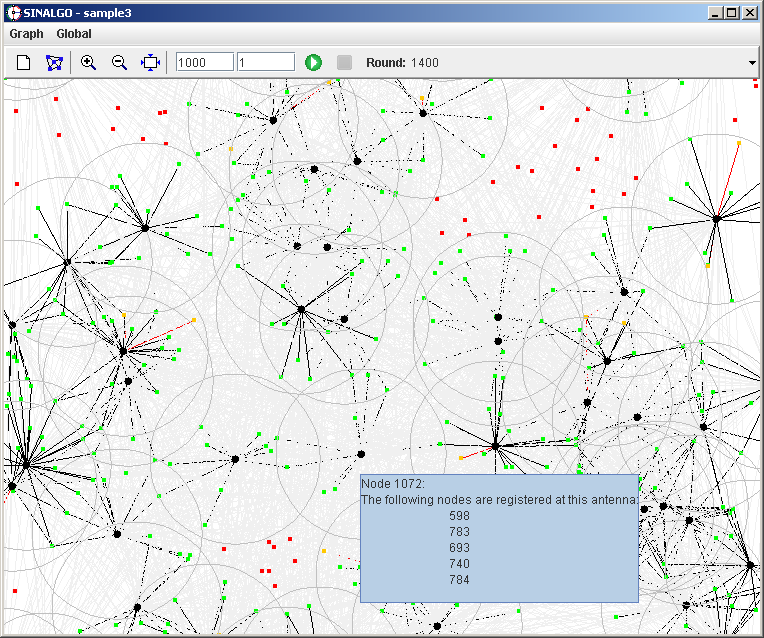
\includegraphics[width=0.22\linewidth]{img/screenshot1}}
\;
\subfigure[][]{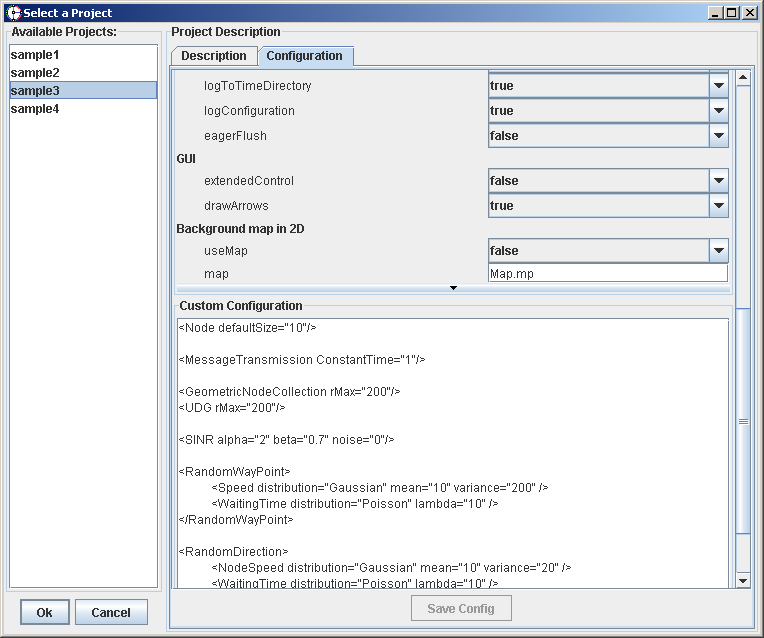
\includegraphics[width=0.22\linewidth]{img/screenshot2}}
\;
\subfigure[][]{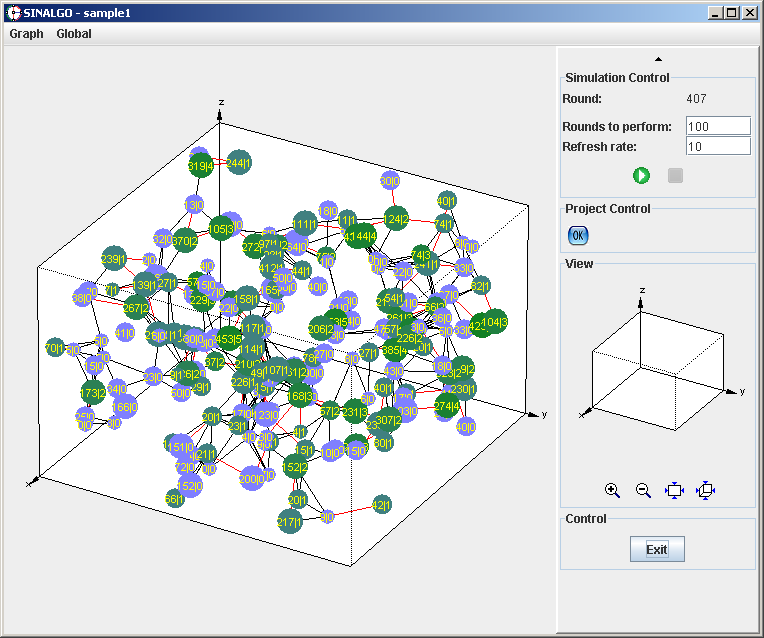
\includegraphics[width=0.22\linewidth]{img/screenshot3}}
\;
\subfigure[][]{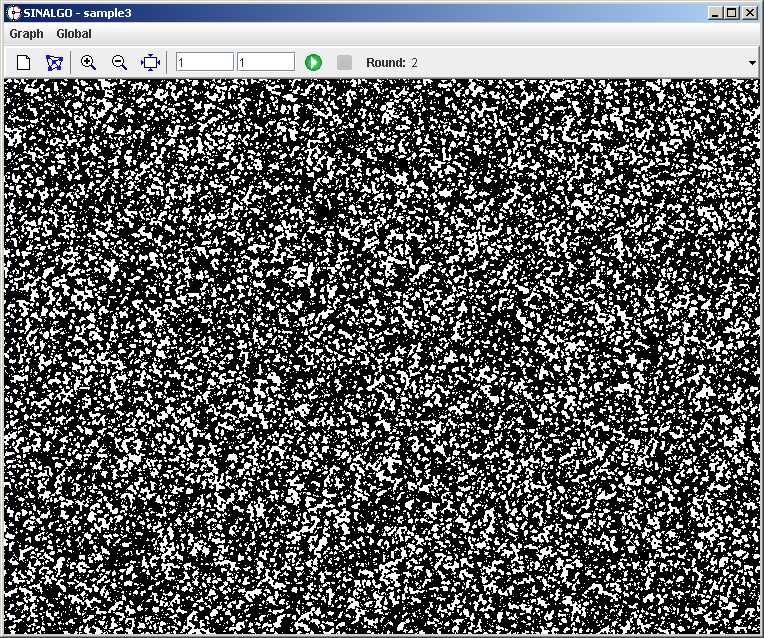
\includegraphics[width=0.22\linewidth]{img/screenshot4}}
%\caption{Imagens lado a lado}

\end{figure}
\end{frame}

%------------------------------------------------

\begin{frame}\frametitle{Introdução}

\begin{block}{Fácil extensão (models)}
\begin{itemize}
	\item Mobilidade.
	\item Conectividade.
	\item Distribuição.
	\item Confiabilidade.
	\item Transmissão de Mensagens.
\end{itemize}
\end{block}

\end{frame}

%------------------------------------------------
\section{Primeros Passos com o Sinalgo} % Sections can be created in order to organize your presentation into discrete blocks, all sections and subsections are automatically printed in the table of contents as an overview of the talk
%------------------------------------------------

\subsection{Ambiente de Desenvolvimento} % A subsection can be created just before a set of slides with a common theme to further break down your presentation into chunks
%------------------------------------------------

\begin{frame}
\frametitle{Getting Started}
\begin{block}{Pré-requisitos}
\begin{itemize}
	\item Java 5.0 (J2SE 5.0 JDK) ou superior.
	\item \href{https://www.eclipse.org/downloads/}{\textcolor{red}{Eclipse}}.
\end{itemize}
\end{block}

\begin{block}{Versões}
\begin{itemize}
	\item \href{http://sourceforge.net/project/showfiles.php?group_id=192227}{\textcolor{red}{Regular Release (recomendo)}}.
	\item \href{http://sourceforge.net/project/showfiles.php?group_id=192227}{Toy Release}.
\end{itemize}
\end{block}
\end{frame}

%------------------------------------------------

\subsection{Instalação e Documentação} % A subsection can be created just before a set of slides with a common theme to further break down your presentation into chunks
%------------------------------------------------

\begin{frame}
\frametitle{Getting Started}

\begin{alertblock}{Como instalar? (Regular Release com Eclipse)}
	\begin{enumerate}
		\item Crie um projeto ('File' $\rightarrow $ 'New' $\rightarrow $ 'Project')
		\item Escolha um projeto do tipo 'Java Project'.
		
		\item Dê um nome de sua preferência (ex: "SinalgoAula").
		
		\item Importe o Sinalgo Regular Release para seu Workspace.
		\begin{enumerate}
			\item Extraia sinalgo-x.xx.x.zip para um diretório temporário
			\item Faça a cópia do conteúdo do Regular Release para o seu projeto
			\item Certifique-se de que o arquivo \textbf{.classpath} foi sobrescrito.
		\end{enumerate}

		\item Verifique se Eclipse está configurado com Java 5.0 ou superior.
		\begin{enumerate}
			\item ('Window' $\rightarrow $ 'Preferences'), 'Java' $\rightarrow $ 'Compiler'
			\item ('Window' $\rightarrow $ 'Preferences'), select 'Java' $\rightarrow $ 'Installed JREs'
		\end{enumerate}
	\end{enumerate}
\end{alertblock}

\begin{itemize}
	\item Mais detalhes... \href{http://disco.ethz.ch/projects/sinalgo/tutorial/Installation.html}{\textbf{Aqui}}.
\end{itemize}


\end{frame}

%------------------------------------------------

\begin{frame}
\frametitle{Getting Started}



\begin{columns}[c] % The "c" option specifies centered vertical alignment while the "t" option is used for top vertical alignment

\column{.6\textwidth} % Left column and width
\begin{exampleblock}{Como executar?}
	\begin{enumerate}
		\item Clique com o botão direito na pasta “src” dentro da aba 
“Project Explorer” ou “Navigator” do Eclipse

		\item Clique na opção “Run As” $\rightarrow $ “Java Application”
		
		\item Na tela “Select Java Application”, selecione a classe “Run”.
		
		\item Mais detalhes sobre  \href{http://disco.ethz.ch/projects/sinalgo/tutorial/Installation.html}{\textbf{instalação}} 
		e 
\href{http://disco.ethz.ch/projects/sinalgo/tutorial/Execution.html}{\textbf{execução}}.
	\end{enumerate}
\end{exampleblock}

\column{.4\textwidth} % Right column and width

\begin{figure}[t]
	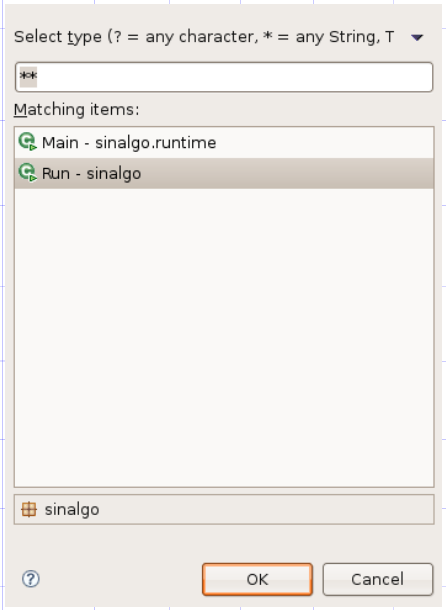
\includegraphics[width=1\linewidth]{img/run}<1>
\end{figure}

\begin{figure}[t]
	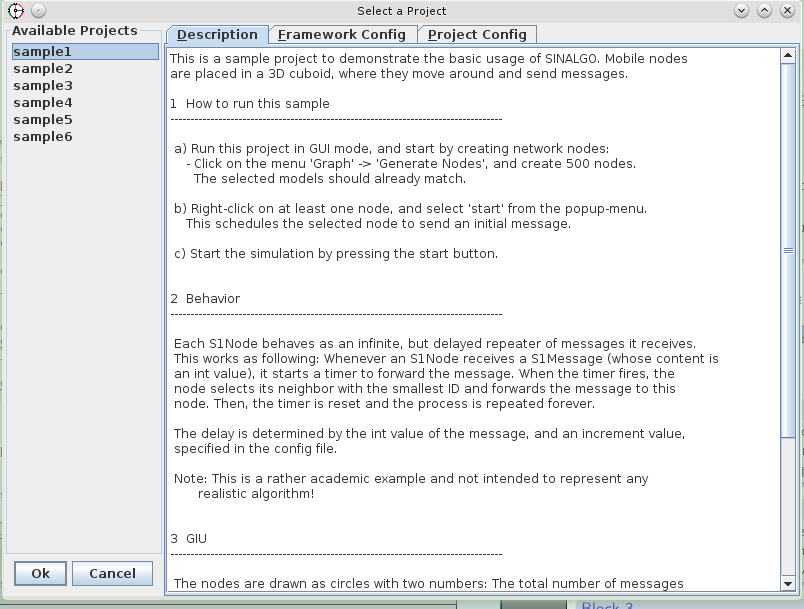
\includegraphics[width=1\linewidth]{img/menu}<2>
	\caption{se tudo deu certo!}
\end{figure}
\end{columns}

\end{frame}

%------------------------------------------------

\begin{frame}
\frametitle{Getting Started}


\begin{columns}[c] % The "c" option specifies centered vertical alignment while the "t" option is used for top vertical alignment

\column{.45\textwidth} % Left column and width
\begin{block}{Documentação}
	\begin{enumerate}
		\item O código é bem documentado
		\begin{enumerate}
			\item Os 6 exemplos podem ser utilizados como base
		\end{enumerate}

		\item \href{http://www.stack.nl/~dimitri/doxygen/}{\textbf{doxygen}}
		
		\item \href{http://disco.ethz.ch/projects/sinalgo/index.html}{\textbf{Sinalgo Site!}}
		
		\item Mais detalhes sobre  \href{http://disco.ethz.ch/projects/sinalgo/tutorial/Installation.html}{\textbf{instalação}} 
		e 
\href{http://disco.ethz.ch/projects/sinalgo/tutorial/Execution.html}{\textbf{execução}}.
	\end{enumerate}
\end{block}

\column{.6\textwidth} % Right column and width

\begin{exampleblock}{}
\begin{figure}[t]
	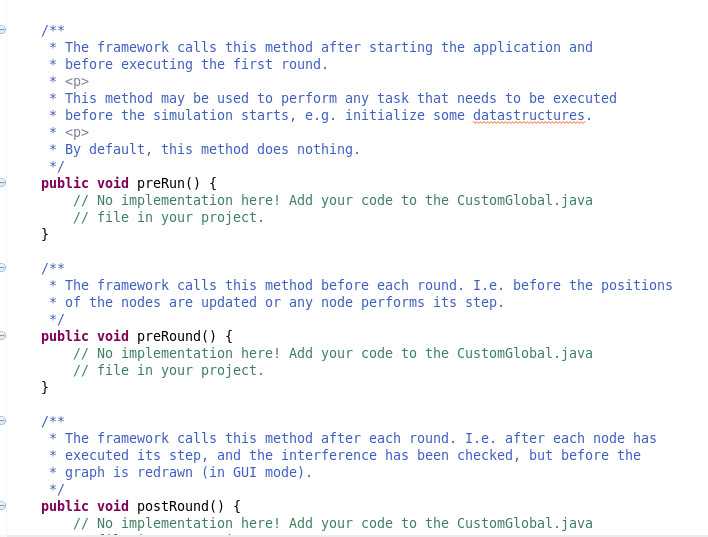
\includegraphics[width=1\linewidth]{img/documentation}
\end{figure}
\end{exampleblock}

\end{columns}

\end{frame}


%------------------------------------------------
\section{Projetos no Sinalgo} % Sections can be created in order to organize your presentation into discrete blocks, all sections and subsections are automatically printed in the table of contents as an overview of the talk
%------------------------------------------------
\subsection{Árvore de Diretório de um Projeto} % Sections can be created in order to organize your presentation into discrete blocks, all sections and subsections are automatically printed in the table of contents as an overview of the talk
%------------------------------------------------

\begin{frame}
	\frametitle{Árvore de diretórios}
\begin{columns}[c] % The "c" option specifies centered vertical alignment while the "t" option is used for top vertical alignment

\column{.7\textwidth} % Left column and width
	\begin{block}{Sinalgo Projects}
	\small
		\begin{itemize}
			\item Sinalgo disponibiliza 6 projetos
			\item Um projeto é uma pasta dentro do diretório 'src/projects/' do Sinalgo
		\end{itemize}
	\end{block}
	
	\begin{exampleblock}{Criando um novo projeto}<2->
	\small
		\begin{enumerate}
			\item Faça uma copia da pasta 'src/projects/template/' para o mesmo diretório
			\item Modifique o nome 'template (copy)' para o nome do seu projeto
			
			\item Execute a aplicação novamente...
						
			\item Pronto!
		\end{enumerate}
	\end{exampleblock}
	
\column{.35\textwidth} % Left column and width

\begin{exampleblock}{}
\begin{figure}[t]
	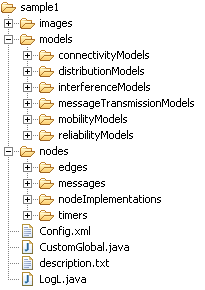
\includegraphics[width=0.8\linewidth]{img/projectFolders}
\end{figure}
\end{exampleblock}

\end{columns}


\end{frame}

%------------------------------------------------

\begin{frame}
	\frametitle{Erros}
	
	\begin{exampleblock}{Erros aos copiar 'src/projects/template/'}
		É normal alguns erros de declaração dos packages.\\
		Para corrigir basta modificar para: \\
		\textbf{package projects.nomeDoSeuProjeto>}
	\end{exampleblock}
	
	\begin{exampleblock}{}<1>
		\begin{figure}[t]
			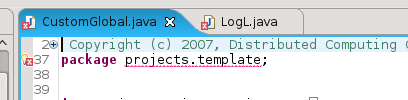
\includegraphics[width=1\linewidth]{img/exemplo-erro}
		\end{figure}
	\end{exampleblock}

	
	
	
\end{frame}
%------------------------------------------------

\begin{frame}
	\frametitle{Dica!}
	
	\begin{alertblock}{}
	Obs: É altamente recomendado gerar um projeto para cada 
algoritmo simulado. Contudo, isso freqüentemente resulta em 
código comum. Ao invés de copiar o mesmo código para todos 
os projetos, é preferível criar um novo projeto que armazenará 
esse código-comum e do qual todos os outros projetos terão 
acesso.
	\end{alertblock}	
	
	
\end{frame}

%------------------------------------------------
\subsection{Criando um Projeto} % Sections can be created in order to organize your presentation into discrete blocks, all sections and subsections are automatically printed in the table of contents as an overview of the talk
%------------------------------------------------

\begin{frame}
	\frametitle{Meu Primeiro Projeto}
	\begin{block}{Exemplo PingPong}<1->
	\justifying
		Vamos criar uma simples simulação que demonstra os conceitos básicos.\\
		 Copie o diretório 'src/projects/template/' e modifique o nome para 'pingPong'
	\end{block}
	
	
	\begin{exampleblock}{Comportamento PingPong}<2->
	\begin{itemize}
		\item Nesta simulação, dois nós vão trocar mensagens entre si.
		\item Os nós geram cores em RGB de modo aleatório.
		\item Cada cor gerada deve ser anexada em uma mensagem, que será enviada para o vizinho.
		\item Ao receber uma mensagem:
		\begin{itemize}
			\item O nó deve alterar sua cor conforme os valores RBG recebidos.
			\item Gerar uma nova cor RGB e enviar por broadcast. 
		\end{itemize}		 
	\end{itemize}
	\end{exampleblock}	
	
	
\end{frame}


%------------------------------------------------

\begin{frame}
	\frametitle{Meu Primeiro Projeto}
	
	\begin{block}{Por onde começo a implementar?}
		R: Em todos projetos temos que implementar:
		\begin{enumerate}
			\item Comportamento do nó
			\item Modelos
			\item Criar um arquivo de configuração
		\end{enumerate}
	\end{block}	
	
\end{frame}

%------------------------------------------------
\subsection{Implementação do Projeto} % Sections can be created in order to organize your presentation into discrete blocks, all sections and subsections are automatically printed in the table of contents as an overview of the talk
%------------------------------------------------

\begin{frame}
	\frametitle{Como implementar o comportamento do nó?}
	
	\begin{block}{Básica implementação}
		\begin{enumerate}
			\item Cada nó simulado é uma instância (sub-classe) da classe \textbf{"sinalgo.nodes.Node"}.
			\item Salve a classe em \textbf{'nodes/nodeImplementations/'} do projeto pingPong.
			\item Cada nó implementa seu próprio comportamento:
			\begin{itemize}
				\item Ex: cada nó tem um método que é chamado quando uma mensagem é recebida. Também existe um método para enviar mensagens para seus vizinhos.
				\item Você deve implementar o comportamento adequado para cada mensagem recebida.
			\end{itemize}
			\item Cada nó tem sua própria instância de Mobilidade, Confiabilidade, Interferência, e Conectividade.
			\item Existe um modelo de Transmissão de Mensagens que é global.
			
		\end{enumerate}
	\end{block}	
	
\end{frame}

%------------------------------------------------

\begin{frame}
	\frametitle{Como implementar o comportamento do nó?}
	
	\begin{block}{Criando um nó}
		\begin{enumerate}
			\item Crie uma classe que estenda \textbf{'sinalgo.nodes.Node'} chamada "PingPongNode.java'.
			\item handleMessages() é o método onde o comportamento deve ser implementado.
		\end{enumerate}
			
	\end{block}	
	
	\begin{alertblock}{OBS}
	Obrigatoriamente, deve-se implementar o método 
handleMessages() e, opcionalmente, qualquer 
um dos métodos abstratos da classe 
sinalgo.nodes.Node
	\end{alertblock}
	
\end{frame}
%------------------------------------------------

\begin{frame}
\tiny
	\lstinputlisting[caption="pingPongNode.java"]{codes/pingPongNode.java}
\end{frame}

%------------------------------------------------
\begin{frame}
	\frametitle{Como implementar o comportamento do nó?}
	
	\begin{block}{Criando uma mensagem}
	\small
		\begin{enumerate}
			\item Antes de implementar o handleMessages(), vamos criar nossa \textbf{Mensagem}.
			\item A comunicação no Sinalgo é feita através de mensagens.
			\item Toda mensagem deve herdar da classe \textbf{'sinalgo.nodes.messages.Message'}
			\item As mensagens devem ser salvas no diretório:
			\begin{itemize}
				\item \textbf{'nodes/messages/'} do projeto pingPong.
				
			\end{itemize}
			
			 \item A classe abstrata Message requer que seja 
implementada apenas um método.
			\begin{itemize}
				\item \textbf{public Message clone( );}
			\end{itemize}
		\end{enumerate}
		
	\end{block}	
	
	
\end{frame}
%------------------------------------------------
\begin{frame}
	\frametitle{Como implementar o comportamento do nó?}
	
	\begin{alertblock}{OBS}
		\textbf{
			Quando um nó envia uma mensagem para um nó vizinho, 
			assume-se que o destino recebe o conteúdo da mensagem que foi 
			enviado pelo método send( ). O framework, contudo, não tem 
			como saber se o transmissor ainda tem uma referência para o 
			objeto de mensagem enviado, e conseqüentemente, ele pode alterar 
			a mensagem enviada. Para enviar tais problemas, o framework 
			envia cópias separadas para todos os nós que recebem uma 
			mensagem.
		}
	\end{alertblock}
	
\end{frame}
%------------------------------------------------

\begin{frame}
\tiny
	\lstinputlisting[caption="PingPongMessage.java"]{codes/PingPongMessage.java}
\end{frame}

%------------------------------------------------



\begin{frame}
\frametitle{Como implementar o comportamento do nó?}
	\begin{block}{Criando uma mensagem}
		\begin{itemize}
			\item A classe é auto-explicativa.
			\item Basicamente definimos os campos da mensagem 
					e a implementação do método clone( ), que será 
					usado para gerar uma cópia da mensagem.
		\end{itemize}
	\end{block}
\end{frame}

%------------------------------------------------



\begin{frame}
	\frametitle{Como implementar o comportamento do nó?}
	
	\begin{block}{Voltando a implementação do nó...}
		\begin{enumerate}
			\item O método mais importante é o handleMessage(Inbox inbox).
			\item handleMessages(Inbox inbox) é o método onde o comportamento deve ser implementado.
			\item Esse método é usado para tratar as mensagens que o nó recebeu.
			\item Cada nó armazena as mensagens que recebe em uma instância da classe Inbox.
			
			\item Inbox provê um iterador para acessar cada mensagem armazenada.
			
			\item Para cada mensagem, o interador armazena meta-informações, como o transmissor (sender) da mensagem.
		\end{enumerate}
			
	\end{block}	
	
\end{frame}

%------------------------------------------------

\begin{frame}
\tiny
	\lstinputlisting[caption="handleMessage"]{codes/handleMessage.java}
\end{frame}

%------------------------------------------------
\begin{frame}
	\frametitle{Como implementar o comportamento do nó?}
	
	\begin{block}{Voltando a implementação do nó...}
		\begin{enumerate}
			\item A classe pingPongNode.java já é capaz de receber e tratar as mensagens recebidas.
			\item \textcolor{red}{\textbf{Mas como mandar mensagens?}}
			\item O que é \textcolor{red}{\textbf{ PingPongTimer?}}
		\end{enumerate}
			
	\end{block}	

\end{frame}

%------------------------------------------------
\begin{frame}
	\frametitle{Como implementar o comportamento do nó?}
	
	\begin{block}{Temporizadores}
		\begin{enumerate}
			\item Temporizadores servem para especificarmos quando uma determinada ação deverá ser executada.
			\item No nosso exemplo, criamos um temporizador com a seguinte declaração:
			\begin{itemize}
				\item \textbf{PingPongTimer timer = new PingPongTimer(pkt);}
				\item Perceba que passamos como parâmetro, para o construtor, a mensagem que queremos transmitir. Mais a frente, explicaremos o porque.
			\end{itemize}
		\end{enumerate}
			
	\end{block}	
	


\end{frame}

%------------------------------------------------
\begin{frame}
	\frametitle{Como implementar o comportamento do nó?}

	\begin{exampleblock}{Considerações}
		\begin{itemize}
			\item Iniciamos o temporizador através do seguinte  comando:
			\begin{itemize}
				\item \textbf{timer.startRelative(1, this);}
				\item O primeiro parâmetro indica em qual turno o temporizador 
será disparado. O segundo parâmetro indica qual objeto  está disparando o temporizador.
				\item O tempo 1 indica que o temporizador será disparado no 
próximo round.
			\end{itemize}
			
		\end{itemize}
	\end{exampleblock}

\end{frame}

%------------------------------------------------
\begin{frame}
	\frametitle{Como implementar o comportamento do nó?}
	
	\begin{block}{Criando um temporizadores}
		\begin{enumerate}
			\item Todo temporizador herda da classe \textbf{'sinalgo.nodes.timers.Timer'}		
			\item Crie uma classe chamada PingPongTimer.java dentro de 'nodes/timers/':
			\item Basicamente, implementamos o método \textbf{fire( )}, que é a ação a ser executada quando o temporizador for disparado.
			
			\item No nosso exemplo, queremos que:
			\begin{itemize}
				\item Toda vez que o temporizador for disparado, ou seja, quando fire() é executado,
				\item o método broadcast do nó que iniciou o temporizador será disparado para enviar a mensagem.
			\end{itemize}
		\end{enumerate}
			
	\end{block}	
	
\end{frame}
%------------------------------------------------

\begin{frame}
\tiny
	\lstinputlisting[caption="PingPongTimer.java"]{codes/PingPongTimer.java}
\end{frame}

%------------------------------------------------
\begin{frame}
	\frametitle{Como implementar o comportamento do nó?}
	
	\begin{block}{Criando um método para iniciar a comunicação}
		\begin{enumerate}
			\item Como iniciar a troca de mensagens?
			\item Adicione o seguinte método na classe PingPongNode.java:
		\end{enumerate}
			
	\end{block}	

\begin{columns}[c]<2-> % The 'c' option specifies centered vertical alignment while the 't' option is used for top vertical alignment

\column{.85\textwidth} % Left column and width

	\lstinputlisting[caption="NodePopupMethod"]{codes/NodePopupMethod.java}

\column{.25\textwidth} % Left column and width
	\begin{exampleblock}{}<3>
		\begin{figure}[t]
			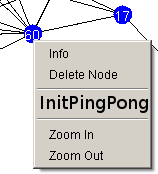
\includegraphics[width=1\linewidth]{img/popup}
		\end{figure}
	\end{exampleblock}

\end{columns}
\end{frame}

%------------------------------------------------
\begin{frame}
	\frametitle{Como implementar o comportamento do nó?}
	
	\begin{block}{Arquivo de configuração}
		\begin{enumerate}
			\item Nossa simulação já está pronta!!!
			\item Falta somente configurar o projeto:
			\begin{itemize}
				\item Edite o arquivo \textbf{pingPong/config.xml}
			\end{itemize}
		\end{enumerate}
	\end{block}	
	
	\lstinputlisting[caption="Config.xml", language=XML]{codes/Config1.xml}
\end{frame}
%------------------------------------------------

\begin{frame}
\tiny
	\lstinputlisting[caption="Config.xml", language=XML]{codes/Config.xml}
\end{frame}
%------------------------------------------------

\begin{frame}
\footnotesize
\centering

	
\includegraphics[width=0.22\linewidth]{img/git.png}
	\begin{exampleblock}{Git é vida!}
		git clone git@github.com:BrunoPereiraSantos/WirelessNetwork-Sinalgo.git
	\end{exampleblock}
	
\end{frame}
%------------------------------------------------
\section{Exercícios} % Sections can be created in order to organize your presentation into discrete blocks, all sections and subsections are automatically printed in the table of contents as an overview of the talk
%------------------------------------------------
\subsection{Exemplos do Sinalgo} % Sections can be created in order to organize your presentation into discrete blocks, all sections and subsections are automatically printed in the table of contents as an overview of the talk
%------------------------------------------------
\begin{frame}
	\frametitle{Tarefa 1}
	
	\begin{alertblock}{Exemplos do Sinalgo}
		\begin{enumerate}
			\item Execute os 6 exemplos do Sinalgo.
			\item Descreva a finalidade do exemplo.
			\item Quais conceitos visto em sala de aula que são demonstrados em cada exemplo.
			\item Descreva as limitações de cada exemplo.
			\item Quais os pontos fortes e fracos do Sinalgo?
		\end{enumerate}
	\end{alertblock}
\end{frame}

%------------------------------------------------
\subsection{Árvore de Roteamento} % Sections can be created in order to organize your presentation into discrete blocks, all sections and subsections are automatically printed in the table of contents as an overview of the talk
%------------------------------------------------
\begin{frame}
	\frametitle{Tarefa 2}
	\small
	\begin{alertblock}{Árvore para coleta de dados}
		\begin{enumerate}
			\item Faça uma inundação para descobrir o menor caminho (em saltos) de cada nó para uma Estação Base (EB).
			\item A EB deve ser iniciada através de \textbf{@NodePopupMethod}
			\item As mensagens podem ser do tipo rota ou dados
			\item O nó deve identificar se a mensagem é de construção de rota ou de dados.
			\begin{itemize}
				\item Se a mensagem é de construção de rota
				\begin{itemize}
					\item O nó deve atualizar sua rota para a EB.
				\end{itemize}
				\item Se a mensagem é de dados
				\begin{itemize}
					\item O nó deve mandar uma mensagem unicast para o próximo salto até a EB, caso exista uma rota válida
				\end{itemize}
			\end{itemize}
			
		\end{enumerate}
	\end{alertblock}
\end{frame}

%------------------------------------------------
\begin{frame}
	\frametitle{Tarefa 2}
	\begin{alertblock}{Árvore para coleta de dados}
		\begin{enumerate}
			
			\item A EB ao receber uma mensagem deve imprimir no Output informações sobre a mensagem coletada.
				
			\item Cada nó após ter um caminho válido para EB, deve ser permitido enviar dados periodicamente (10 rounds) para EB, isto deve ser ativado através de um \textbf{@NodePopupMethod}.  

			\item O payload da mensagem de dado pode ser uma amostra de temperatura ou alguma variável de ambiente geralmente analisada por RSSF.
			
			\item A mensagem não pode trafegar mais que um tempo de vida estabelecido (Ex: 30 saltos)
		\end{enumerate}
	\end{alertblock}
\end{frame}

%------------------------------------------------
\begin{frame}
	\frametitle{Tarefa 2}
	\begin{block}{DICAS}
		\begin{enumerate}
			\item Use Tools.java para:
			\begin{itemize}
				\item Escrever no output
				\item Manipular erros
				\item Informações sobre a simulação
				\item Acessar conjunto de nós
				\item Acessar mensagens
				\item Usar métodos relacionados com a GUI
				\item Parar a simulação
			\end{itemize}
			\item Como mandar mensagens unicast? 
			\begin{itemize}
				\item R: documentação sinalgo! =D
			\end{itemize}
		\end{enumerate}
	\end{block}
\end{frame}

%------------------------------------------------
\begin{frame}
	\frametitle{Tarefa 2}
	\begin{block}{DICAS}
		\begin{enumerate}
			\item Quais classes devo criar?
			\begin{itemize}
				\item Uma classe para representar o nó (Ex: "MyNode.java")
				\begin{itemize}
					\item A classe deve conter uma referência para o próximo salto até a EB.
					\item Deve ter uma variável para indicar sua distância até a EB.
					\item Criar um método menu popup para iniciar a EB na classe "MyNode.java".
					\item Implemente um mecanismo para evitar loop das mensagens (Dica: use o campo número de saltos da mensagem)
				\end{itemize}
			\end{itemize}
		\end{enumerate}
	\end{block}
\end{frame}

%------------------------------------------------
\begin{frame}
	\frametitle{Tarefa 2}
	\begin{block}{DICAS}
		\begin{enumerate}
			\item Quais classes devo criar?
			\begin{itemize}
				\item Uma ou duas classes para representar as mensagens (rota e dados)
				\item Cabeçalho indicado: 
				\begin{itemize}
					\item número de seqüência.
					\item tempo de vida.
					\item destino e origem.
					\item nó que encaminhou a mensagem
					\item número de saltos até a EB
					\item tipo (se fez uma classe só)
				\end{itemize}
			\end{itemize}
		\end{enumerate}
	\end{block}
\end{frame}

%------------------------------------------------
\begin{frame}
	\frametitle{Tarefa 2}
	\begin{block}{DICAS}
		\begin{enumerate}
			\item Quais classes devo criar?
			\begin{itemize}
				\item Um ou dois timers para enviar as mensagens do flood (para descoberta das rotas) e para enviar periodicamente as mensagens de dados.
				\item Implementar um temporizador que armazene um pacote.
				\item implementar adequadamente o método \textbf{fire()}.
			\end{itemize}
		\end{enumerate}
	\end{block}
\end{frame}

%------------------------------------------------
\begin{frame}
\begin{center}
	Até a próxima aula!
\end{center}
	
\end{frame}


%----------------------------------------------------------------------------------------

\end{document} 